% intro
In this section a background is given on the theory used in order to implement Bayesian co-evolution. It is divided into four parts, namely rare controllable events, neural networks, gaussian processes and (co)evolution. 

\subsection{Controllable rare events}
%Kern is goed, maar moet wat strakker geformuleerd worden. Eventueel terminologie uit de presentatie gebruiken? 
% Dit nu goed (ik nam aan dat met presentatie de proposal was bedoeld)??
Figure \ref{rareControllableImage} illustrates the concept of controllable rare events with two policies. Rare events are those of which the chance of occurring is very small, while an event is controllable when the choice of policy affects the performance greatly. A controllable rare event is thus an event of which the probability of occurring is low while the chosen action significantly influences the reward.

\begin{figure}[h]
  \centering
  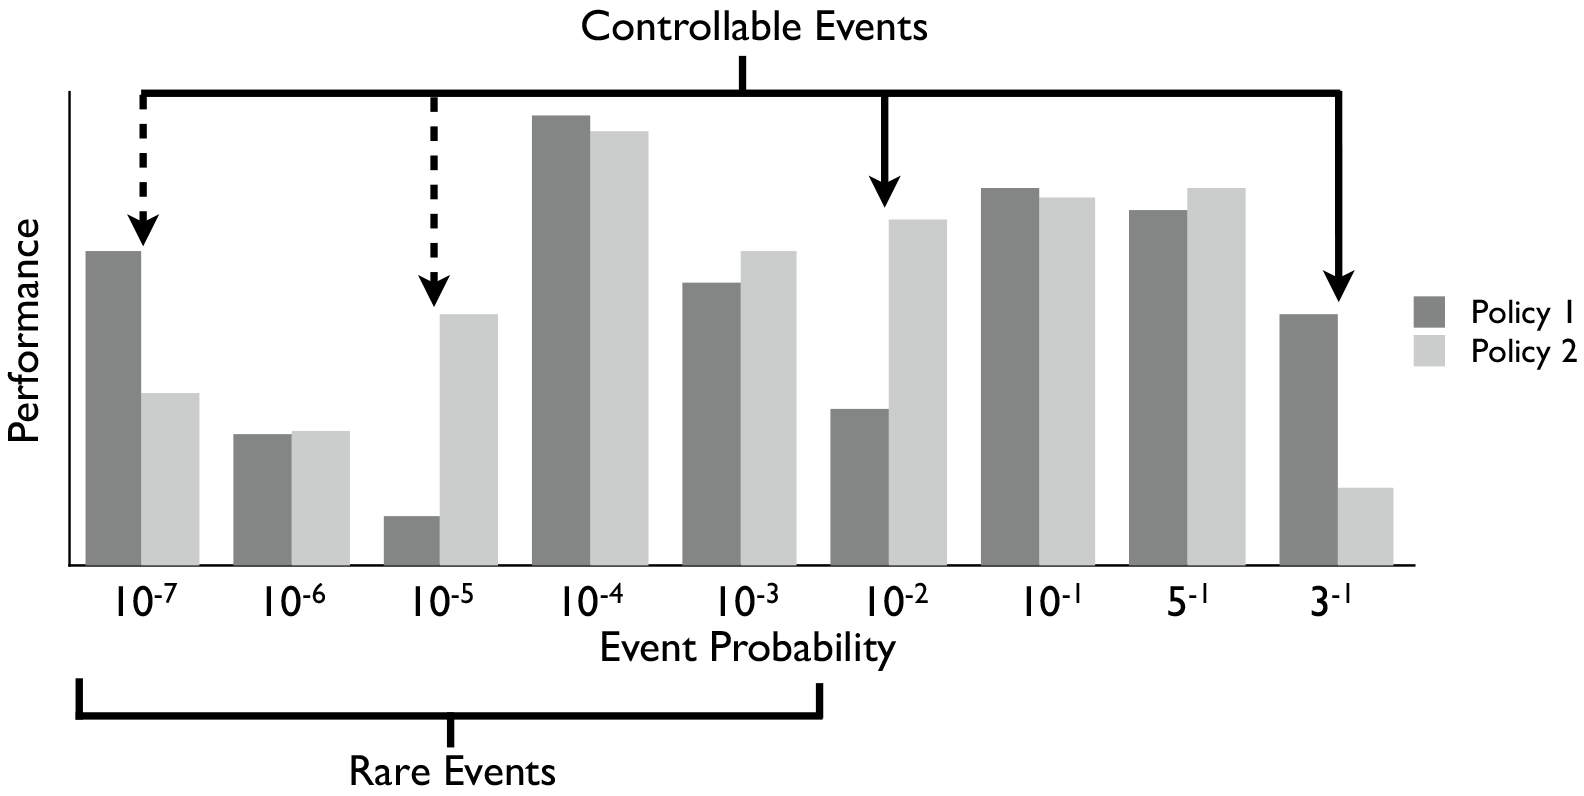
\includegraphics{images/rare-controllable.png}
  \caption{Performance of two policies on a set of events, showing rare-, controllable- and rare controllable events}\label{rareControllableImage}
\end{figure}

Coping properly with events that are both rare and controllable is vital because these events influence the performance of policies while difficult to discover: general approaches tend to ignore rare events. By explicitly focussing on controllable rare events, policies with seemingly equal performance are properly distinguished and the learning process accelerates.

\subsection{Neural Networks}
% meer in detail propagation uitleggen, or bias?
Neural networks are inspired by the central nervous systems and describe a set of nodes of which the (one-directional) connection contain weights. Nodes can be of three types: input-, output- or hidden nodes. The input nodes receive a signal (value), which are propagated to the next layer of nodes by multiplication with the corresponding weights. The values are propagated through the network and eventually reach the output nodes, which defines the output of the network. 

Neural networks are viable options as representation for policies. In such a situation the input of the network is often the state of the world, while the output describes the action taken (given this state).

\subsection{Gaussian Process}
% TODO

GP is used to maintain a believe over the fitness of policies and evolution is used as a means to do policy search.

\subsection{(Co) evolution}
% our context -> evolution bridge
In the process of creating a better believe of the fitness over the policies, a method is required to define new policies. In order to do so, evolutionary algorithms are used. 

% evolution
Evolutionary algorithms aim to produce new entities based on a population and is inspired by biological evolution. Given a set of organisms, offspring is born by applying crossover and mutation operators, by combining the genes of the parents the new individuals exhibit similar, but slightly different, features. The selection of parents is based on an evaluation of the original set of organisms, and the better performing offspring replaces the least suited parents. 

% evolution -> our context finish
% including bias?
When applied to neural networks, the set of weights of the network represents one organism in the population. The weights are then evolved as described above.

% co evolution 
Co evolution is the act of evolving two populations while their evaluation depends on the other population. A classical example is in a prey-predator context. The fitness of an individual depends on its survivability (either ability to hunt prey or evade predators) and the more fit a parent is, the more likely it produces offspring. \\

% outro
In the following section (\ref{related}) the related work will be described, followed by our contribution (\ref{contrib}). We then describe the experiments (\ref{experiments}), discuss them and lastly conclude (\ref{conclusion}).

